\begin{quote}
	\textit{``If the chaos of the nineties reflects a radical shift in the paradigms of visual literacy, the final shift away from the Lascaux/Gutenberg tradition of a pre-holographic society, what should we expect from this newer technology, with his promise of discrete encoding and subsequent reconstruction of the full range of sensory perception?''}
\end{quote}
\hfill \textit{Burning Chrome, William Gibson}
\\
\\

%=========================================================================================================

Introduction goes here.

%=========================================================================================================

Contributions (as laid out in intro, but elaborate? or maybe have them in their entirety in both places)

%=========================================================================================================

Future work

%=========================================================================================================

Final Thoughts

final quote?

%=========================================================================================================



\begin{figure}[h]
	\begin{center}
		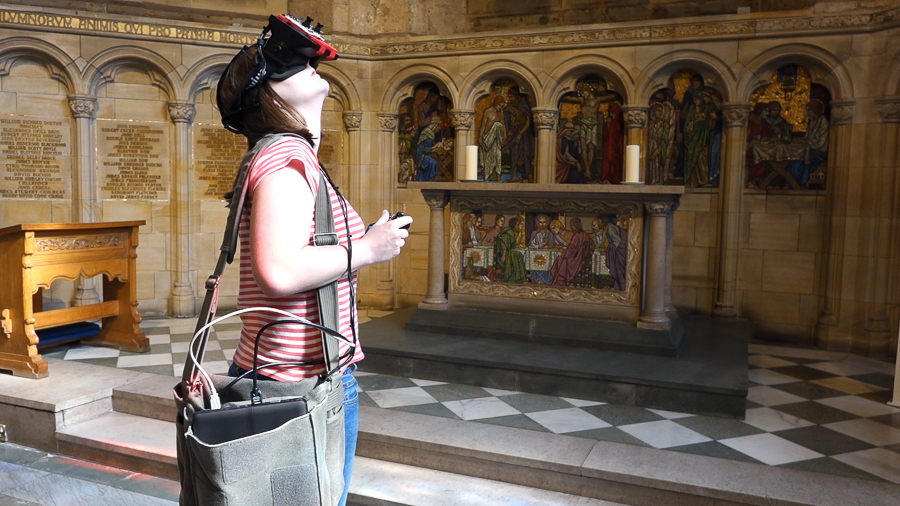
\includegraphics[width=\textwidth]{participant-f-4.jpg}
		\caption{The \textit{Mirrorshades} parallel reality platform in use.}
		\label{participant-f-4.jpg}
	\end{center}	
\end{figure}









%=========================================================================================================

\section{Summary}


\begin{itemize}
	\item 
	\item 
	\item 
	\item 
	\item 
	\item 
	\item 
	\item 
	\item 
	\item 
\end{itemize}


\section{PR Best Practices}

\begin{itemize}
	\item A 100\% RW view \& a 100\% VR view should be provided
	\item A method of transitioning between the two views at a user-controlled speed, with the ability to pause at any inbetween balance, should be provided
	\item A default view with \textless than 100\% RW should be provided, but should be toggleable \& not enforced
	\item This \textless 100\% should not be too much \textless 100\% because going too far hampers the overall experience
\end{itemize}




\section{Future Work}

Gear VR style hardware